\documentclass[12pt,english]{article}

\usepackage[a4paper,
            bindingoffset=0.2in,
            left=1in,
            right=1in,
            top=1in,
            bottom=1in,
            footskip=.25in]{geometry}

% % Set page size and margins
% % Replace `letterpaper' with`a4paper' for UK/EU standard size
% \usepackage[letterpaper,top=2cm,bottom=2cm,left=3cm,right=3cm,marginparwidth=1.75cm]{geometry}
\topmargin=-.3in \oddsidemargin=.3in \evensidemargin=.3in \textheight=9in \textwidth=6in

\usepackage{tikz}
\usepackage{pgfplots}
\usepackage{float}
\usepackage{adjustbox}
\usepackage{multirow}
\usepackage{hhline}

\usepackage{algorithm, algpseudocode}
\usepackage{setspace}

\algrenewcommand\textproc{}

\algnewcommand\algorithmicswitch{\textbf{switch}}
\algnewcommand\algorithmiccase{\textbf{case}}
\algnewcommand\algorithmicassert{\texttt{assert}}
\algnewcommand\Assert[1]{\State \algorithmicassert(#1)}%
% New "environments"
\algdef{SE}[SWITCH]{Switch}{EndSwitch}[1]{\algorithmicswitch\ #1\ \algorithmicdo}{\algorithmicend\ \algorithmicswitch}%
\algdef{SE}[CASE]{Case}{EndCase}[1]{\algorithmiccase\ #1}{\algorithmicend\ \algorithmiccase}%
\newcommand{\pluseq}{\mathrel{{+}{=}}}
\algblockdefx[Foreach]{Foreach}{EndForeach}[1]{\textbf{foreach} #1 \textbf{do}}{\textbf{end foreach}}


% \newcommand{\makeheight}[1]{%
%   \settoheight{\dimen0}{T}% a capital letter
%   \rule[-\dimexpr(#1-\dimen0)/2]{0pt}{#1}%
% }

\newcommand{\myindent}[1]{
\newline\makebox[#1cm]{}
}

\usepackage{amsmath}





\title{\textbf{Hadith Movement}}
\date{}

\begin{document}
\maketitle

\section{Hadith to Edges}
\vspace*{-0.4cm}
\hspace*{-2cm}
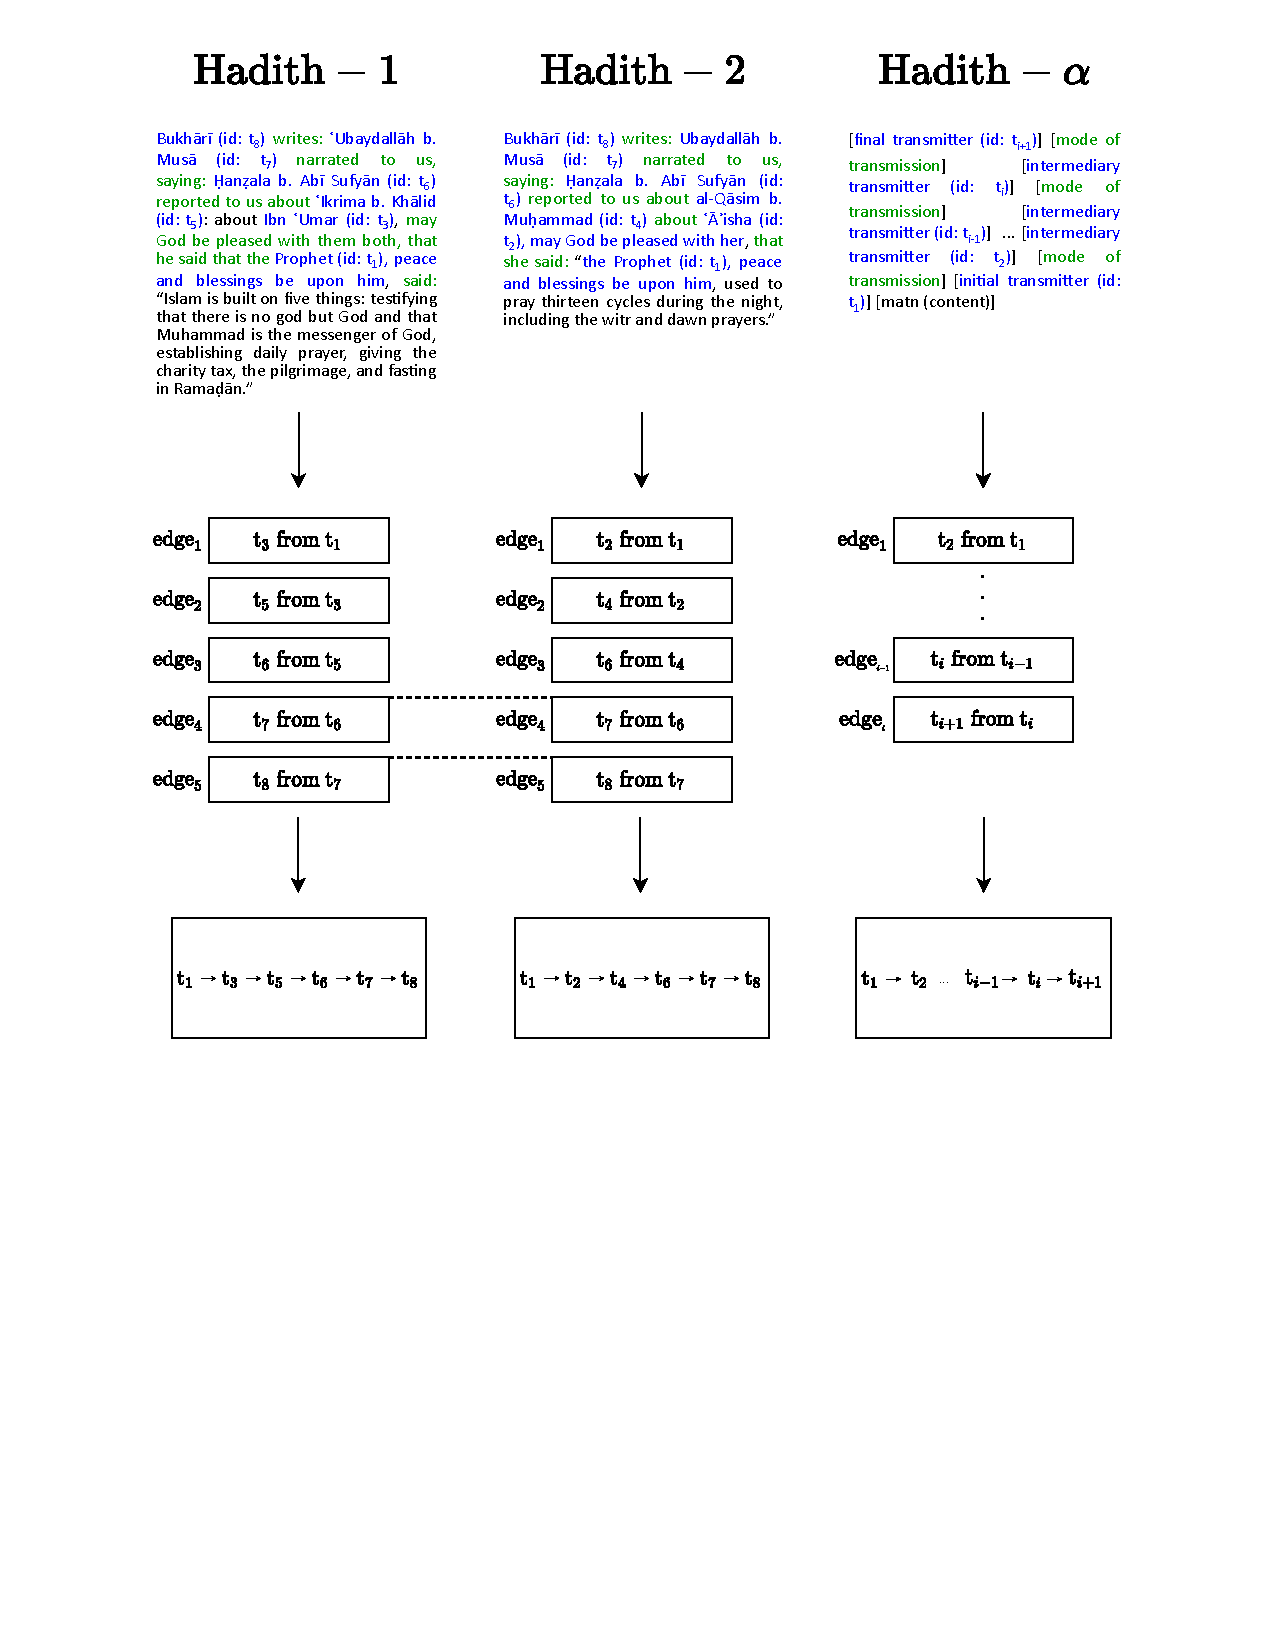
\includegraphics[scale=0.9]{hadith-to-edges/b0_hadith_to_edges.pdf}

\newpage
\section{Edges to HSN}
% \begin{figure}[ht]
% \begin{center}
\vspace*{-0.4cm}
\hspace*{-2cm}
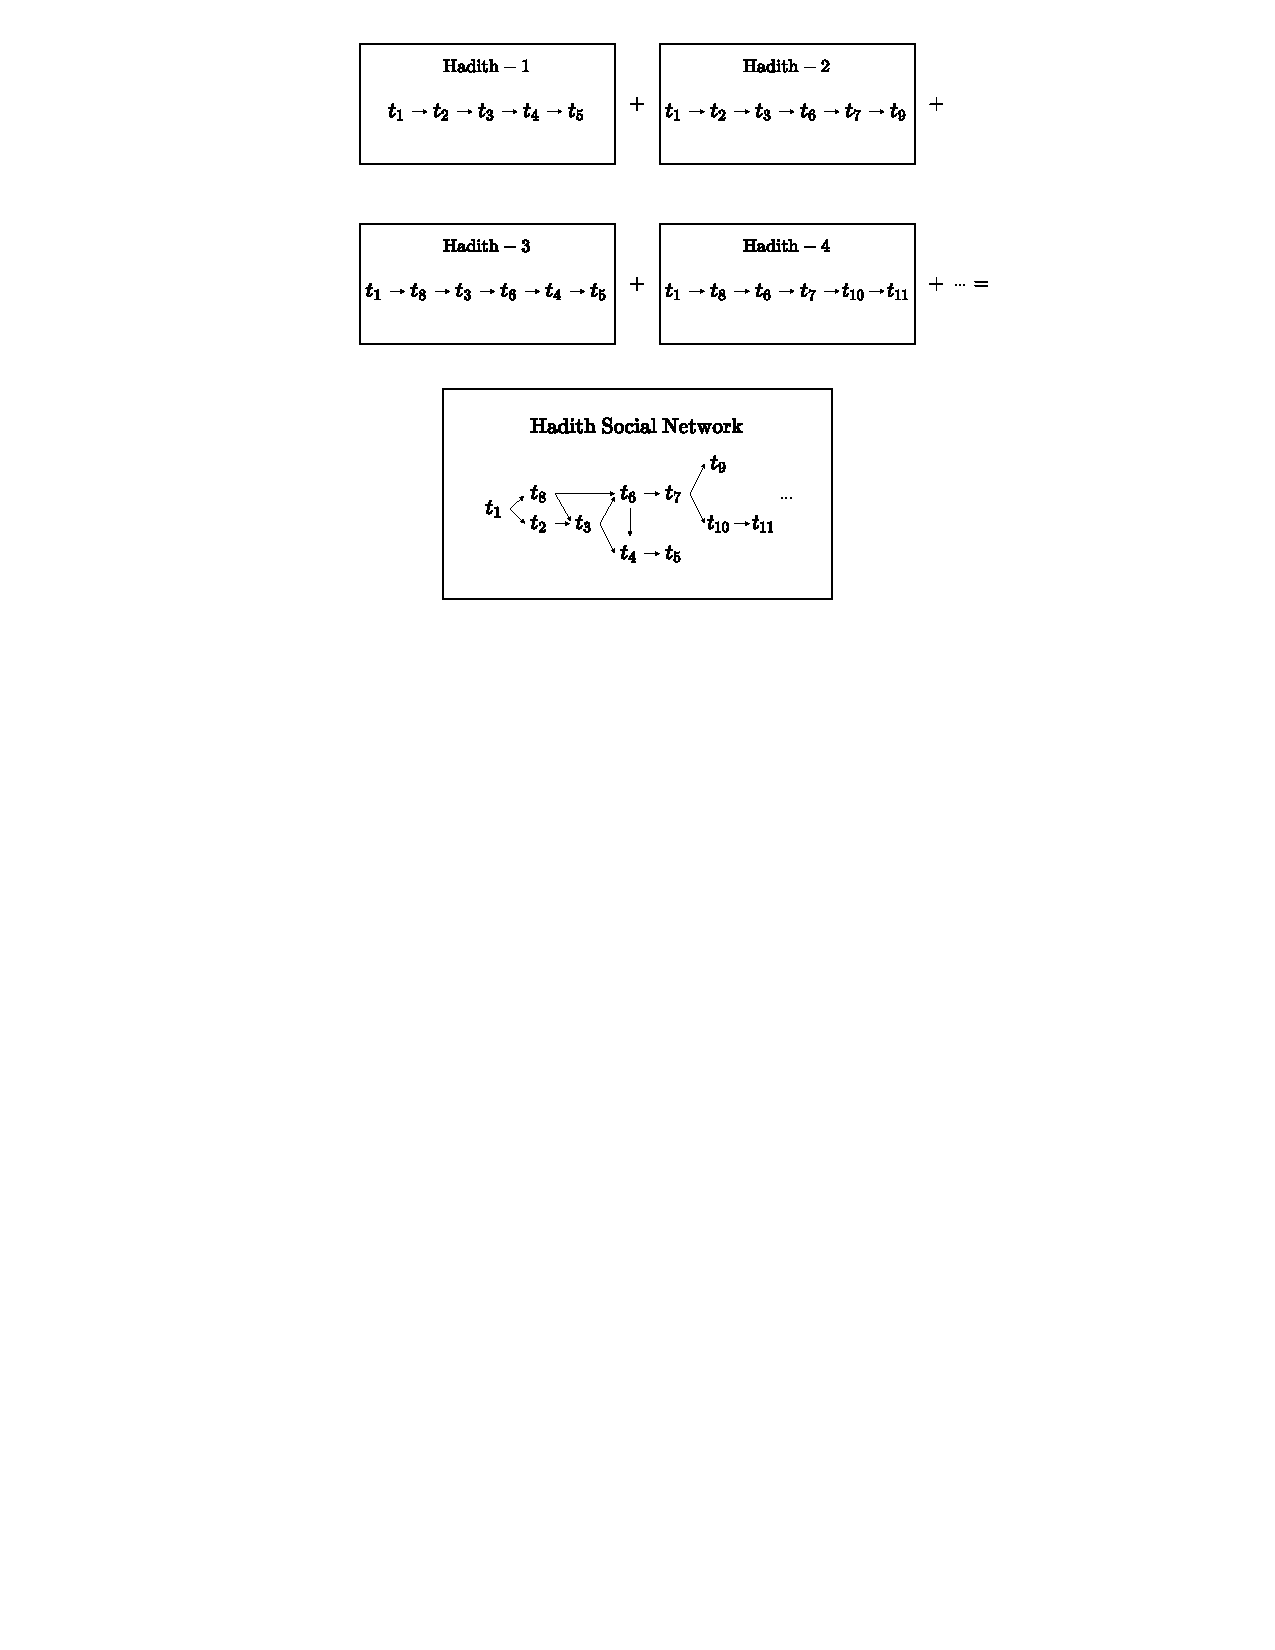
\includegraphics[scale=0.9]{edges-to-hsn/b1_edges_to_hsn.pdf}
% \end{center}
% \end{figure}

\newpage
\section{Travel Analysis}
\subsection{Number of Transmitters in each Isnad}

\begin{adjustbox}{center}
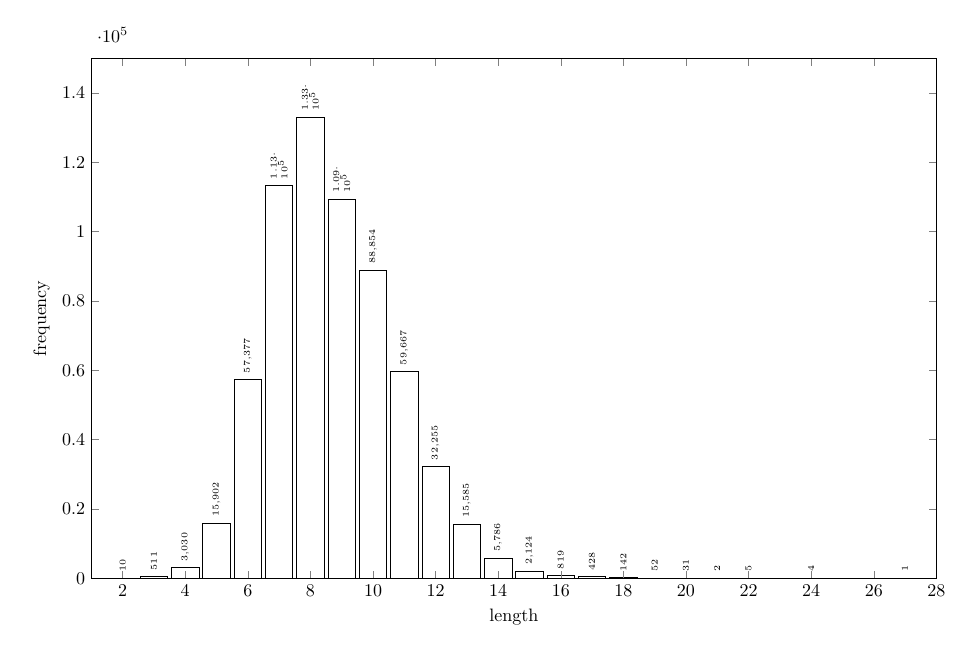
\begin{tikzpicture}[scale=.65]
\begin{axis}[%
xlabel = length,
ylabel = frequency,
scale only axis,
width=6.5in,
height=4in,
nodes near coords,
nodes near coords style={font=\tiny, rotate=90, anchor=west, text width=.03cm},
xmin=1, xmax=28,
ymin=0, ymax=150000,
axis on top]
\addplot[
  ybar,
  bar width=0.2105in, 
  bar shift=0in,
  fill=white,
  draw=black] 
  plot coordinates{ 
  (2, 10) (3, 511) (4, 3030) (5, 15902) (6, 57377) (7, 113327) (8, 132996) (9, 109329) (10, 88854) (11, 59667) (12, 32255) (13, 15585) (14, 5786) (15, 2124) (16, 819) (17, 428) (18, 142) (19, 52) (20, 31) (21, 2) (22, 5) (24, 4) (27, 1)
  };
\end{axis}
\end{tikzpicture}
\end{adjustbox}

\newpage

\subsection{Travel Duration of each Hadith}

\begin{adjustbox}{center}
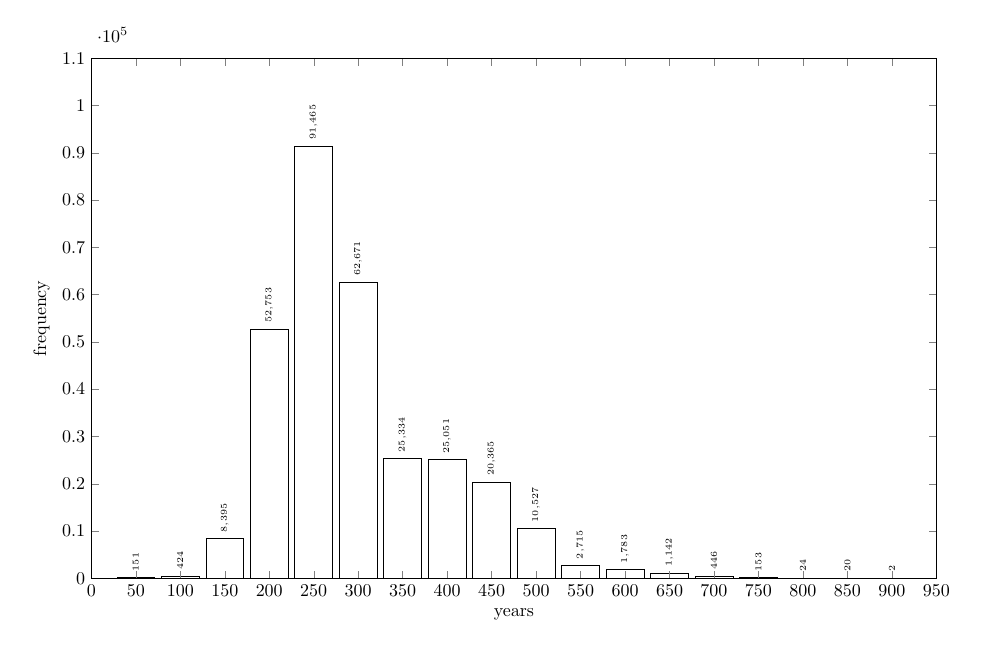
\begin{tikzpicture}[scale=.65]
\begin{axis}[%
xlabel = years,
ylabel = frequency,
scale only axis,
width=6.5in,
height=4in,
nodes near coords,
nodes near coords style={font=\tiny, rotate=90, anchor=west, text width=.03cm},
xmin=0, xmax=950,
ymin=0, ymax=110000,
axis on top]
\addplot[
  ybar,
  bar width=0.2905in, 
  bar shift=0in,
  fill=white,
  draw=black]
  plot coordinates{ 
  (50, 151) (100, 424) (150, 8395) (200, 52753) (250, 91465) (300, 62671) (350, 25334) (400, 25051) (450, 20365) (500, 10527) (550, 2715) (600, 1783) (650, 1142) (700, 446) (750, 153) (800, 24) (850, 20) (900, 2)
  };
\end{axis}
\end{tikzpicture}
\end{adjustbox}


\newpage

\subsection{Number of Cities in each Transmitter's Biography}

\begin{adjustbox}{center}
\begin{tikzpicture}[scale=.65]
\begin{axis}[%
xlabel = cities,
ylabel = frequency,
scale only axis,
width=6.5in,
height=4in,
nodes near coords,
nodes near coords style={font=\tiny, rotate=90, anchor=west, text width=.03cm},
xmin=0, xmax=22,
ymin=0, ymax=20000,
axis on top]
\addplot[
  ybar,
  bar width=0.2705in, 
  bar shift=0in,
  fill=white,
  draw=black]
  plot coordinates{ 
  (1, 15741) (2, 5490) (3, 1501) (4, 442) (5, 210) (6, 97) (7, 59) (8, 35) (9, 14) (10, 8) (11, 8) (12, 8) (13, 6) (14, 4) (15, 1) (16, 2) (19, 1) (21, 3)
  };
\end{axis}
\end{tikzpicture}
\end{adjustbox}

\newpage
\section{City Analysis}
\begin{table}[H]
\centering
\begin{tabular}{|l|c|}
\hline
\multirow{2}{1cm}{city}&\multirow{2}{2cm}{\centering biography count}\\
& \\
\hline
bghdad & 4,966 \\
\hline
dmshq & 3,533 \\
\hline
bsrh & 3,136 \\
\hline
kwfh & 2,802 \\
\hline
almdynh & 2,209 \\
\hline
msr & 1,744 \\
\hline
sham & 1,191 \\
\hline
asbhan & 1,144 \\
\hline
nysabwr & 1,068 \\
\hline
mkh & 965 \\
\hline
mrw & 586 \\
\hline
alhjaz & 506 \\
\hline
alry & 503 \\
\hline
wast & 476 \\
\hline
hms & 471 \\
\hline
khrasan & 429 \\
\hline
jrjan & 339 \\
\hline
qzwyn & 273 \\
\hline
hrah & 267 \\
\hline
hlb & 257 \\
\hline
al'eraq & 244 \\
\hline
bkhara & 237 \\
\hline
hran & 206 \\
\hline
almwsl & 205 \\
\hline
alymn & 201 \\
\hline
\end{tabular}
\quad
\begin{tabular}{|l|c|}
\hline
\multirow{2}{1cm}{city}&\multirow{2}{2.3cm}{\centering transmission count}\\
&\\
\hline
bsrh & 187,293 \\
\hline
bghdad & 173,657 \\
\hline
kwfh & 158,428 \\
\hline
almdynh & 131,375 \\
\hline
msr & 65,989 \\
\hline
dmshq & 54,425 \\
\hline
nysabwr & 43,123 \\
\hline
mkh & 37,688 \\
\hline
asbhan & 23,323 \\
\hline
wst & 17,686 \\
\hline
mrw & 15,774 \\
\hline
hms & 14,429 \\
\hline
sn'ea' & 13,376 \\
\hline
alry & 7,911 \\
\hline
qrtbh & 6,806 \\
\hline
hran & 5,439 \\
\hline
bghlan & 4,302 \\
\hline
hrah & 4,140 \\
\hline
alrqh & 3,067 \\
\hline
jrjan & 2,921 \\
\hline
aljzyrh & 2,757 \\
\hline
almwsl & 2,542 \\
\hline
bkhara & 2,503 \\
\hline
nsa & 2,135 \\
\hline
aylh & 1,916 \\
\hline
\end{tabular}
\quad
\begin{tabular}{|l|c|}
\hline
\multirow{2}{1cm}{city}&\multirow{2}{2.3cm}{\centering transmission count}\\
&\\
\hline
bsrh & 187,293 \\
\hline
bghdad & 173,657 \\
\hline
kwfh & 158,428 \\
\hline
almdynh & 131,375 \\
\hline
msr & 65,989 \\
\hline
dmshq & 54,425 \\
\hline
nysabwr & 43,123 \\
\hline
mkh & 37,688 \\
\hline
asbhan & 23,323 \\
\hline
wast & 17,686 \\
\hline
mrw & 15,774 \\
\hline
hms & 14,429 \\
\hline
sn'ea' & 13,376 \\
\hline
alry & 7,911 \\
\hline
qrtbh & 6,806 \\
\hline
hran & 5,439 \\
\hline
bghlan & 4,302 \\
\hline
hrah & 4,140 \\
\hline
alrqh & 3,067 \\
\hline
jrjan & 2,921 \\
\hline
almwsl & 2,542 \\
\hline
bkhara & 2,503 \\
\hline
hlb & 1,878 \\
\hline
tws & 1,323 \\
\hline
\multicolumn{2}{c}{} \\
\end{tabular}
\end{table}

\newpage
\section{Edges to City Network}
% \begin{figure}[ht]
% \begin{center}
\vspace*{-0.4cm}
\hspace*{-2cm}
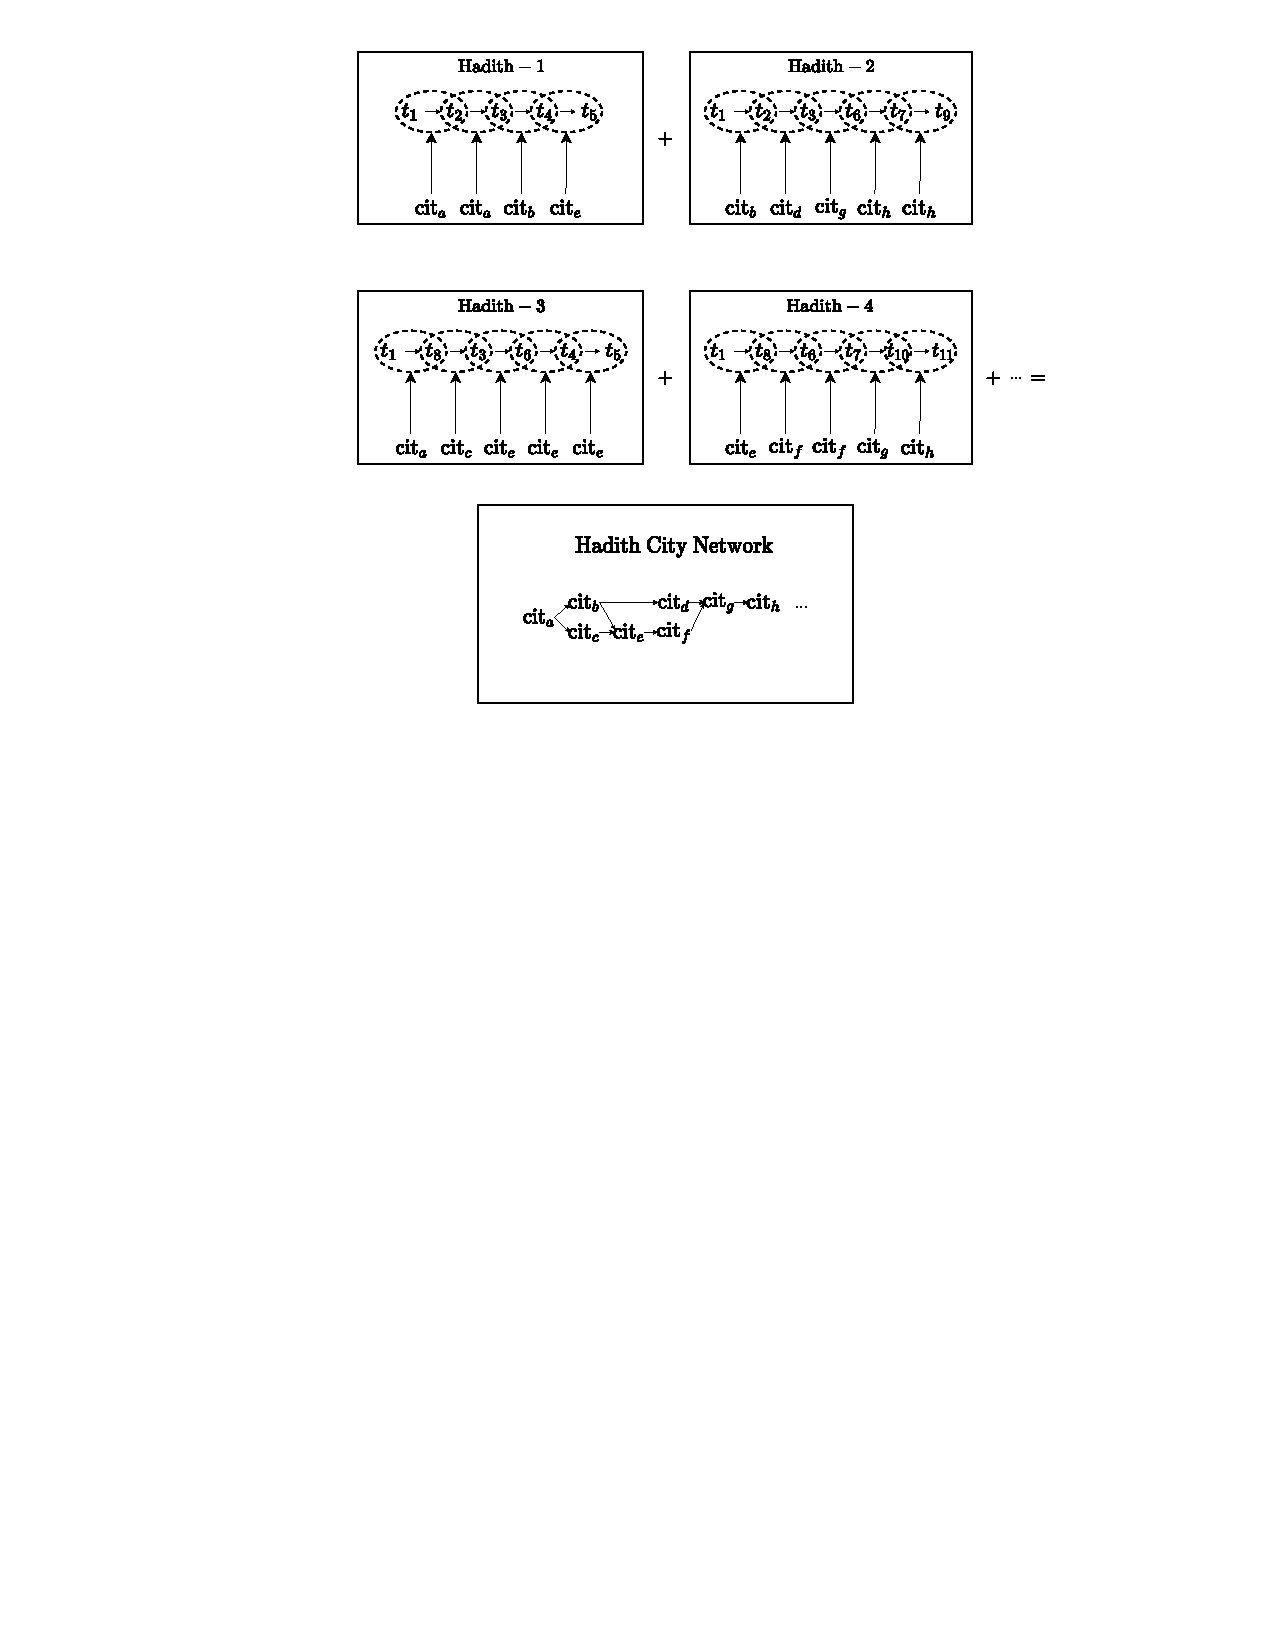
\includegraphics[scale=0.9]{edges-to-city-network/b2_edges_to_city_network.pdf}
% \end{center}
% \end{figure}

\newpage
\section{Top 24 Outgoing Paths in Entire City Network (nodes as cities)}
\vspace*{-3cm}
\hspace*{-4cm}
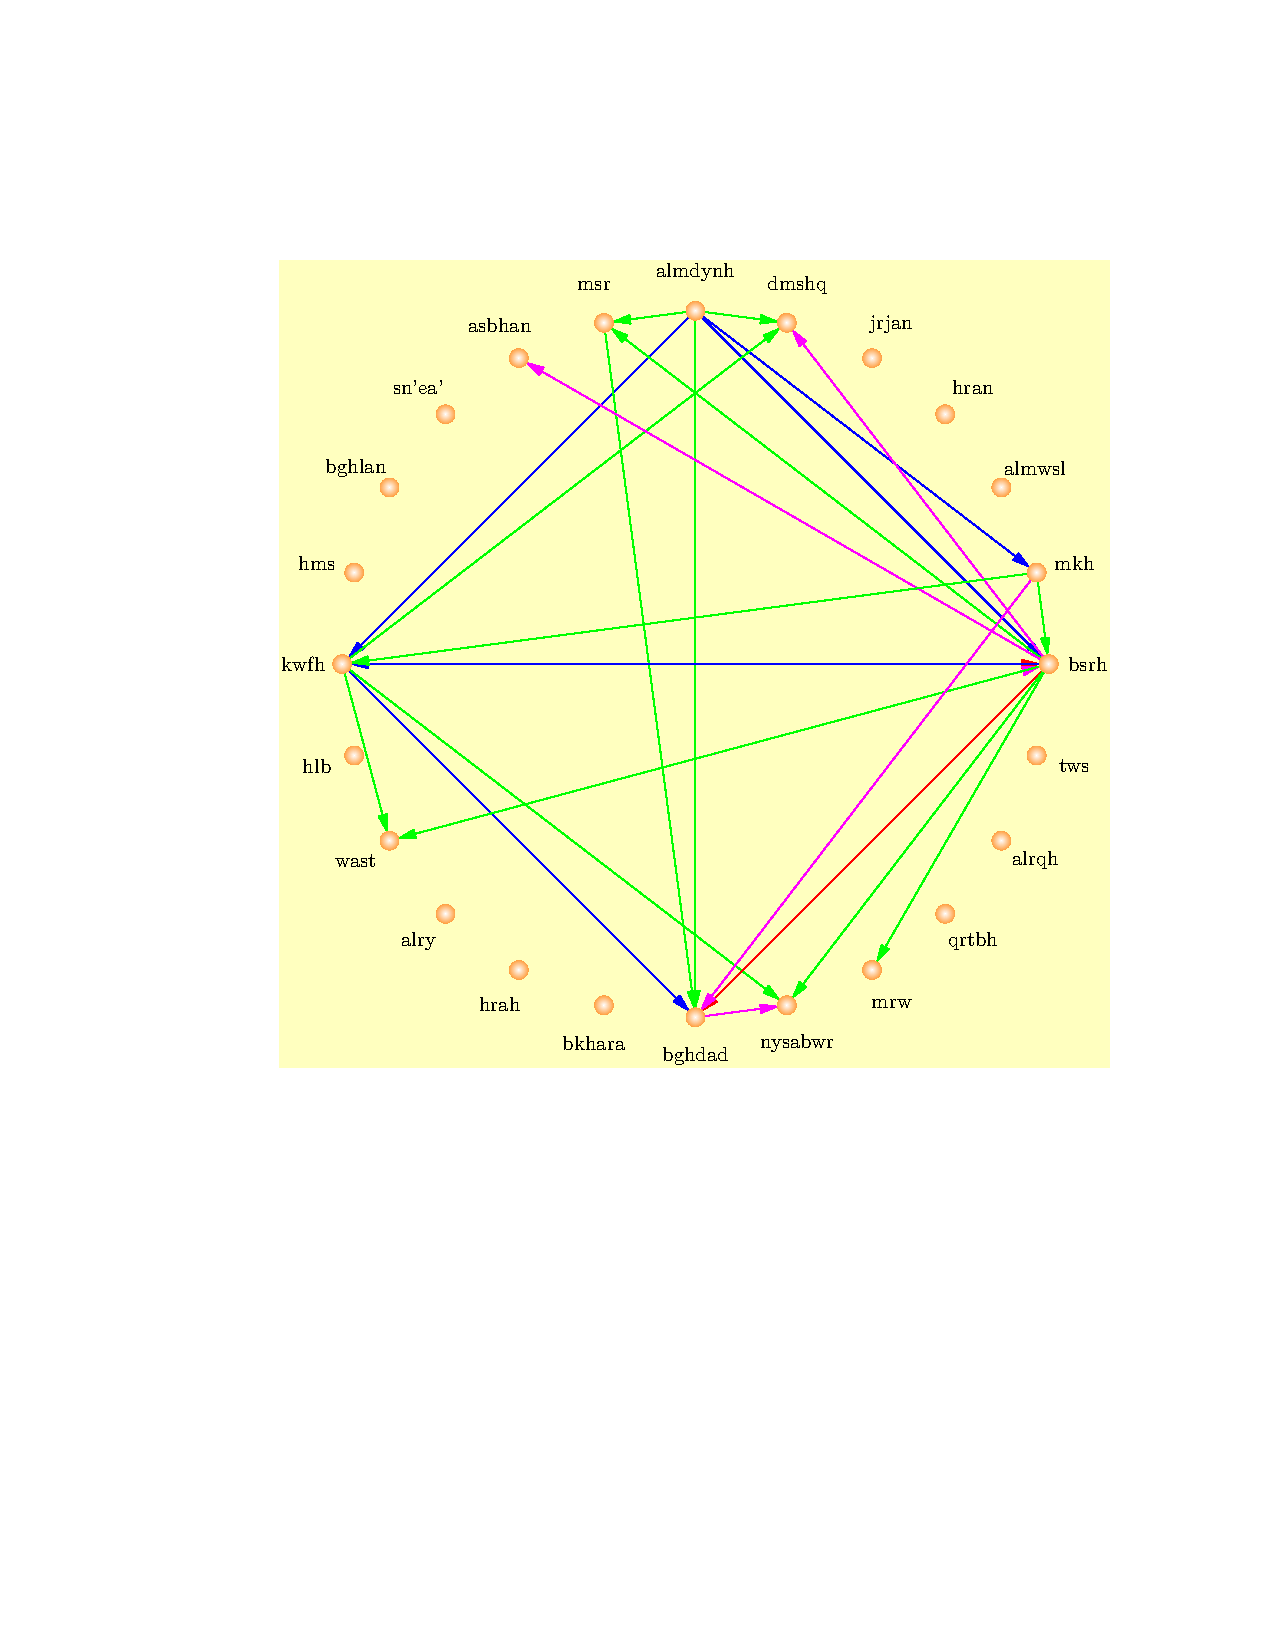
\includegraphics[scale=1]{top-paths/Hadith_Movement_Dragon_Diagram_Top_24_Paths.pdf}

\newpage
\section{Top Outgoing Path from Each City in City Network (nodes as cities)}
\vspace*{-3cm}
\hspace*{-4cm}
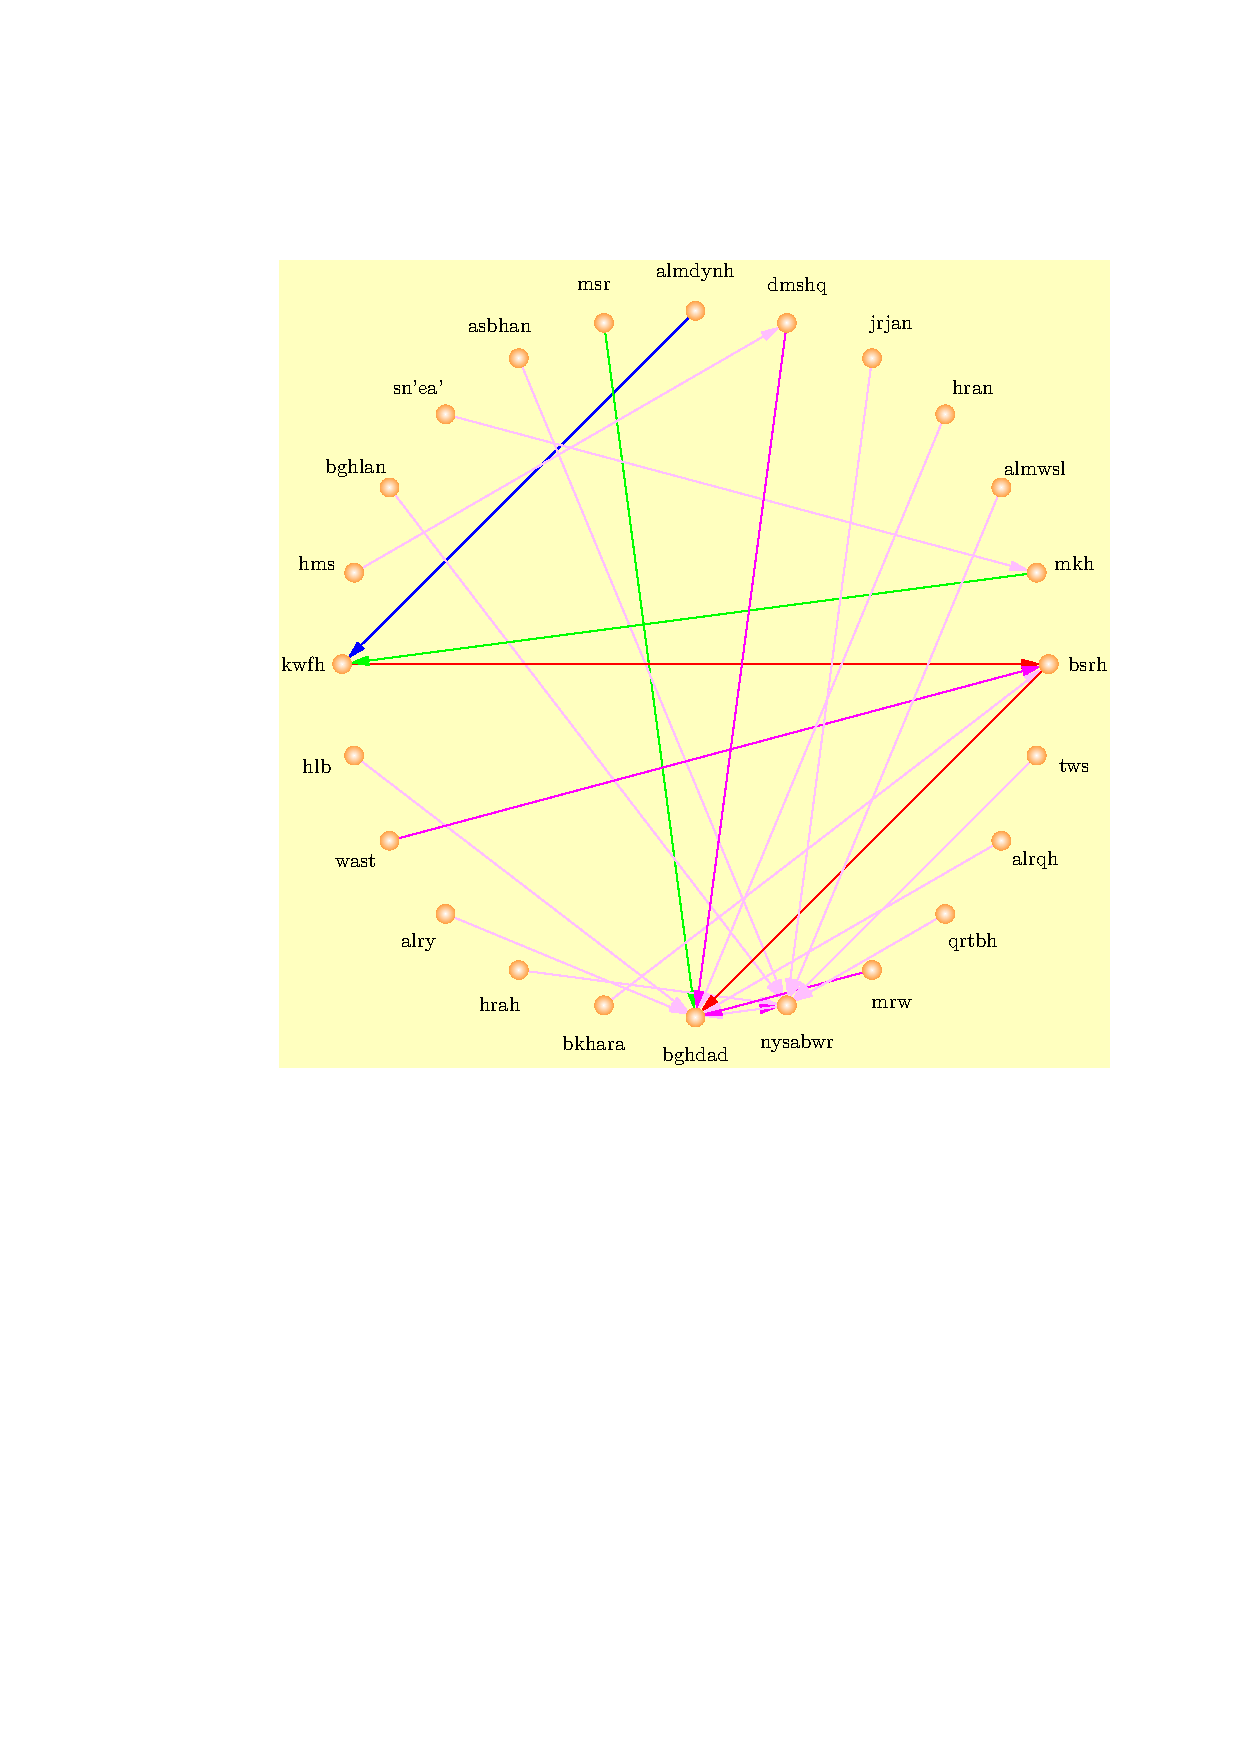
\includegraphics[scale=1]{top-paths/Hadith_Movement_Dragon_Diagram_Top_Path_Out_of_Each_City.pdf}


\newpage
\section{Top 10 Paths in City Network (nodes as cities) in Each 30 Year Partitioned Network}

\begin{table}[H]
\footnotesize
\centering
\resizebox{15cm}{!}{%
\begin{tabular}{ |p{1.6cm}|p{1.6cm}|r||p{1.6cm}|p{1.6cm}|r||p{1.6cm}|p{1.6cm}|r|}
 \hhline{---||---||---}
         \multicolumn{3}{|c||}{\rule{0pt}{.4cm} $-11$ --- 30} &  \multicolumn{3}{c||}{\rule{0pt}{.4cm} 30 --- 60} &
         \multicolumn{3}{c|}{\rule{0pt}{.4cm} 60 --- 90}  \\ 
        %  \cline{1-9}
  \hhline{---||---||---}
 From & To    & Count &  From & To  & Count &  From & To  & Count\\
  \hhline{---||---||---}
almdynh & almdynh & 3798 & almdynh & almdynh & 16053 & almdynh & almdynh & 14248 \\ 
almdynh & kwfh & 2274 & almdynh & kwfh & 2157 & kwfh & kwfh & 3950 \\
almdynh & dmshq & 264 & almdynh & mkh & 1746 & almdynh & mkh & 2565 \\
almdynh & mkh & 208 & almdynh & bsrh & 1164 & almdynh & kwfh & 1885 \\ 
almdynh & hms & 201 & kwfh & kwfh & 1011 & almdynh & bsrh & 1061 \\ 
almdynh & bsrh & 38 & almdynh & dmshq & 423 & bsrh & bsrh & 1024 \\ 
kwfh & kwfh & 37 & almdynh & hms & 394 & mkh & mkh & 1010 \\ 
almdynh & msr & 27 & almdynh & msr & 373 & almdynh & hms & 733 \\ 
almdynh & alhjaz & 27 & almdynh & mrw & 178 & mkh & kwfh & 538 \\ 
almdynh & alrbdh & 22 & mkh & mkh & 68 & almdynh & dmshq & 286 \\ 
  \hhline{===::===::===}
         \multicolumn{3}{|c||}{\rule{0pt}{.4cm} 90 --- 120} &  \multicolumn{3}{c||}{\rule{0pt}{.4cm} 120 --- 150} &
         \multicolumn{3}{c|}{\rule{0pt}{.4cm} 150 --- 180}  \\ 
 \hhline{---||---||---}
 From & To   & Count &  From & To  & Count &  From & To  & Count\\
 \hhline{---||---||---}
almdynh & almdynh & 16002 & kwfh & kwfh & 20461 & bsrh & bsrh & 28105 \\ 
bsrh & bsrh & 7733 & almdynh & almdynh & 16475 & kwfh & kwfh & 20811 \\ 
kwfh & kwfh & 7145 & bsrh & bsrh & 16309 & almdynh & almdynh & 14733 \\ 
almdynh & mkh & 2724 & kwfh & bsrh & 3860 & kwfh & bsrh & 10413 \\ 
mkh & mkh & 2666 & almdynh & kwfh & 3765 & msr & msr & 6306 \\ 
almdynh & bsrh & 2449 & mkh & kwfh & 3145 & almdynh & kwfh & 3500 \\ 
almdynh & dmshq & 1771 & mkh & mkh & 2971 & almdynh & bsrh & 2945 \\ 
almdynh & kwfh & 1209 & almdynh & bsrh & 2874 & almdynh & bghdad & 2838 \\ 
mkh & kwfh & 777 & mkh & sn'ea' & 1918 & wast & bsrh & 2832 \\ 
kwfh & bsrh & 754 & msr & msr & 1847 & bsrh & kwfh & 2374 \\ 
  \hhline{===::===::===}
         \multicolumn{3}{|c||}{\rule{0pt}{.4cm} 180 --- 210} &  \multicolumn{3}{c||}{\rule{0pt}{.4cm} 210 --- 240} &
         \multicolumn{3}{c|}{\rule{0pt}{.4cm} 240 --- 270}  \\ 
 \hhline{---||---||---}
 From & To    & Count &  From & To  & Count &  From & To  & Count\\
 \hhline{---||---||---}
kwfh & kwfh & 30458 & bsrh & bsrh & 35677 & bsrh & bsrh & 15641 \\ 
bsrh & bsrh & 30108 & kwfh & kwfh & 25904 & msr & msr & 10576 \\ 
bsrh & bghdad & 7452 & bghdad & bghdad & 9959 & kwfh & kwfh & 9345 \\ 
msr & msr & 7120 & bsrh & bghdad & 9312 & bghdad & bghdad & 5970 \\ 
sn'ea' & sn'ea' & 5862 & msr & msr & 6688 & bsrh & bghdad & 4436 \\ 
kwfh & bsrh & 5563 & kwfh & bghdad & 5841 & kwfh & bghdad & 3425 \\ 
kwfh & bghdad & 4947 & kwfh & dmshq & 5584 & bsrh & msr & 3147 \\ 
almdynh & msr & 4676 & dmshq & dmshq & 3481 & bsrh & nysabwr & 2403 \\ 
almdynh & bsrh & 4365 & almdynh & almdynh & 3401 & dmshq & dmshq & 2082 \\ 
almdynh & almdynh & 4035 & kwfh & bsrh & 3167 & mkh & mkh & 1466 \\ 
  \hhline{===::===::===}
         \multicolumn{3}{|c||}{\rule{0pt}{.4cm} 270 --- 300} &  \multicolumn{3}{c||}{\rule{0pt}{.4cm} 300 --- 330} &
         \multicolumn{3}{c|}{\rule{0pt}{.4cm} 330 --- 360}  \\ 
         
 \hhline{---||---||---}
 From & To    & Count &  From & To  & Count &  From & To  & Count\\
 \hhline{---||---||---}
bghdad & bghdad & 8837 & bghdad & bghdad & 9271 & bghdad & bghdad & 10419 \\ 
bsrh & bsrh & 7288 & bsrh & bghdad & 2206 & nysabwr & nysabwr & 2537 \\ 
bsrh & bghdad & 6910 & kwfh & bghdad & 1993 & dmshq & dmshq & 1488 \\ 
kwfh & bghdad & 2968 & nysabwr & nysabwr & 1825 & bghdad & asbhan & 1458 \\ 
dmshq & dmshq & 2429 & bsrh & bsrh & 1582 & dmshq & asbhan & 1327 \\ 
msr & msr & 2408 & msr & msr & 1089 & msr & asbhan & 1179 \\ 
mrw & bghdad & 1666 & bsrh & nysabwr & 1086 & bghdad & nysabwr & 1097 \\ 
mkh & bghdad & 1395 & bghdad & almwsl & 1056 & msr & bghdad & 1061 \\ 
bsrh & mkh & 1333 & dmshq & dmshq & 1025 & asbhan & asbhan & 1020 \\ 
nysabwr & nysabwr & 1296 & bghdad & bsrh & 922 & msr & nysabwr & 941 \\ 
 \hhline{---||---||---}
\end{tabular}
}
\end{table}

\newpage
\section{Network Flow (main cities)}
\begin{tikzpicture}[scale=.9]
\begin{axis}[
    xmin = -11, xmax = 410,
    ymin = 0, ymax = 10,
    xtick distance = 50,
    ytick distance = 1,
    minor tick num = 1,
    major grid style = {lightgray},
    minor grid style = {lightgray!25},
    width = \textwidth,
    height = \textwidth,
    legend cell align = {left},
    legend pos = north west,
    axis lines = left,
    xlabel={mot year},
    ylabel={mot ratio}
]
\addplot[blue, only marks, mark=o] table [x=x, y=y, col sep=comma] {network-flow/a4_network_flow_almdynh.csv};
\addplot[green, only marks, mark=o] table [x=x, y=y, col sep=comma] {network-flow/a4_network_flow_bghdad.csv};
\addplot[red, only marks, mark=o] table [x=x, y=y, col sep=comma] {network-flow/a4_network_flow_bsrh.csv};
\addplot[yellow, only marks, mark=o] table [x=x, y=y, col sep=comma] {network-flow/a4_network_flow_kwfh.csv};
% \addplot[red, only marks, mark=o] table [x=x, y=y, col sep=comma] {network-flow/a4_network_flow_dmshq.csv};
% \addplot[yellow, only marks, mark=o] table [x=x, y=y, col sep=comma] {network-flow/a4_network_flow_msr.csv};
% \addplot[purple, only marks, mark=o] table [x=x, y=y, col sep=comma] {network-flow/a4_network_flow_nysabwer.csv};

\end{axis}
\end{tikzpicture}


\newpage
\section{Network Flow (supporting cities)}
\begin{tikzpicture}[scale=.9]
\begin{axis}[
    xmin = -11, xmax = 410,
    ymin = 0, ymax = 10,
    xtick distance = 50,
    ytick distance = 1,
    minor tick num = 1,
    major grid style = {lightgray},
    minor grid style = {lightgray!25},
    width = \textwidth,
    height = \textwidth,
    legend cell align = {left},
    legend pos = north west,
    axis lines = left,
    xlabel={mot year},
    ylabel={mot ratio}
]
\addplot[blue, only marks, mark=o] table [x=x, y=y, col sep=comma] {network-flow/a4_network_flow_mkh.csv};
\addplot[red, only marks, mark=o] table [x=x, y=y, col sep=comma] {network-flow/a4_network_flow_msr.csv};
\addplot[orange, only marks, mark=o] table [x=x, y=y, col sep=comma] {network-flow/a4_network_flow_nysabwr.csv};
\addplot[green, only marks, mark=o] table [x=x, y=y, col sep=comma] {network-flow/a4_network_flow_dmshq.csv};
\addplot[yellow, only marks, mark=o] table [x=x, y=y, col sep=comma] {network-flow/a4_network_flow_asbhan.csv};
\addplot[pink, only marks, mark=o] table [x=x, y=y, col sep=comma] {network-flow/a4_network_flow_wast.csv};

\end{axis}
\end{tikzpicture}


\newpage
\section{Centrality Metrics}
\centering
\begin{tabular}{p{1cm}p{1cm}|p{2cm}|p{2cm}|p{2cm}|p{2cm}|}
\cline{3-6}
& & \multicolumn{4}{ c| }{Centrality Metrics} \\
\cline{3-6}
& & \multicolumn{2}{ |c| }{PageRank} & \multicolumn{2}{ c| }{Betweeness} \\
\cline{1-6}
\multicolumn{1}{ |c| }{From} & \multicolumn{1}{ |c }{To} & \multicolumn{1}{ |c| }{City} & \multicolumn{1}{ |c| }{Value} & \multicolumn{1}{ |c| }{City} & \multicolumn{1}{ |c| }{Value} \\ \cline{1-6}
\multicolumn{1}{ |c| }{-11} & \multicolumn{1}{ |c| }{30} & \multicolumn{1}{ |c| }{almdynh} & \multicolumn{1}{ |c| }{0.0878} & \multicolumn{1}{ |c| }{almdynh} & \multicolumn{1}{ |c| }{192.567} \\ \cline{1-6}
\multicolumn{1}{ |c| }{30} & \multicolumn{1}{ |c| }{60} & \multicolumn{1}{ |c| }{mkh} & \multicolumn{1}{ |c| }{0.065} & \multicolumn{1}{ |c| }{almdynh} & \multicolumn{1}{ |c| }{595.083} \\ \cline{1-6}
\multicolumn{1}{ |c| }{60} & \multicolumn{1}{ |c| }{90} & \multicolumn{1}{ |c| }{almdynh} & \multicolumn{1}{ |c| }{0.0568} & \multicolumn{1}{ |c| }{almdynh} & \multicolumn{1}{ |c| }{901.914} \\ \cline{1-6}
\multicolumn{1}{ |c| }{90} & \multicolumn{1}{ |c| }{120} & \multicolumn{1}{ |c| }{msr} & \multicolumn{1}{ |c| }{0.0579} & \multicolumn{1}{ |c| }{almdynh} & \multicolumn{1}{ |c| }{1212.98} \\ \cline{1-6}
\multicolumn{1}{ |c| }{120} & \multicolumn{1}{ |c| }{150} & \multicolumn{1}{ |c| }{kwfh} & \multicolumn{1}{ |c| }{0.0441} & \multicolumn{1}{ |c| }{bsrh} & \multicolumn{1}{ |c| }{1767.34} \\ \cline{1-6}
\multicolumn{1}{ |c| }{150} & \multicolumn{1}{ |c| }{180} & \multicolumn{1}{ |c| }{kwfh} & \multicolumn{1}{ |c| }{0.0426} & \multicolumn{1}{ |c| }{bsrh} & \multicolumn{1}{ |c| }{2570.18} \\ \cline{1-6}
\multicolumn{1}{ |c| }{180} & \multicolumn{1}{ |c| }{210} & \multicolumn{1}{ |c| }{bghdad} & \multicolumn{1}{ |c| }{0.0416} & \multicolumn{1}{ |c| }{kwfh} & \multicolumn{1}{ |c| }{4151.41} \\ \cline{1-6}
\multicolumn{1}{ |c| }{210} & \multicolumn{1}{ |c| }{240} & \multicolumn{1}{ |c| }{bghdad} & \multicolumn{1}{ |c| }{0.0466} & \multicolumn{1}{ |c| }{bghdad} & \multicolumn{1}{ |c| }{4248.02} \\ \cline{1-6}
\multicolumn{1}{ |c| }{240} & \multicolumn{1}{ |c| }{270} & \multicolumn{1}{ |c| }{bghdad} & \multicolumn{1}{ |c| }{0.0479} & \multicolumn{1}{ |c| }{bghdad} & \multicolumn{1}{ |c| }{5816.34} \\ \cline{1-6}
\multicolumn{1}{ |c| }{270} & \multicolumn{1}{ |c| }{300} & \multicolumn{1}{ |c| }{bghdad} & \multicolumn{1}{ |c| }{0.0464} & \multicolumn{1}{ |c| }{bghdad} & \multicolumn{1}{ |c| }{6749.24} \\ \cline{1-6}
\multicolumn{1}{ |c| }{300} & \multicolumn{1}{ |c| }{330} & \multicolumn{1}{ |c| }{bghdad} & \multicolumn{1}{ |c| }{0.0686} & \multicolumn{1}{ |c| }{bghdad} & \multicolumn{1}{ |c| }{9006.63} \\ \cline{1-6}
\multicolumn{1}{ |c| }{330} & \multicolumn{1}{ |c| }{360} & \multicolumn{1}{ |c| }{bghdad} & \multicolumn{1}{ |c| }{0.0654} & \multicolumn{1}{ |c| }{bghdad} & \multicolumn{1}{ |c| }{8021.82} \\ \cline{1-6}
\multicolumn{1}{ |c| }{360} & \multicolumn{1}{ |c| }{390} & \multicolumn{1}{ |c| }{bghdad} & \multicolumn{1}{ |c| }{0.0639} & \multicolumn{1}{ |c| }{bghdad} & \multicolumn{1}{ |c| }{6961.39} \\ \cline{1-6}
\multicolumn{1}{ |c| }{390} & \multicolumn{1}{ |c| }{420} & \multicolumn{1}{ |c| }{bghdad} & \multicolumn{1}{ |c| }{0.0622} & \multicolumn{1}{ |c| }{bghdad} & \multicolumn{1}{ |c| }{4431.1} \\ \cline{1-6}
\multicolumn{1}{ |c| }{420} & \multicolumn{1}{ |c| }{450} & \multicolumn{1}{ |c| }{dmshq} & \multicolumn{1}{ |c| }{0.0744} & \multicolumn{1}{ |c| }{bghdad} & \multicolumn{1}{ |c| }{3401.95} \\ \cline{1-6}
\multicolumn{1}{ |c| }{450} & \multicolumn{1}{ |c| }{480} & \multicolumn{1}{ |c| }{bghdad} & \multicolumn{1}{ |c| }{0.068} & \multicolumn{1}{ |c| }{bghdad} & \multicolumn{1}{ |c| }{2772.14} \\ \cline{1-6}
\multicolumn{1}{ |c| }{480} & \multicolumn{1}{ |c| }{510} & \multicolumn{1}{ |c| }{bghdad} & \multicolumn{1}{ |c| }{0.0843} & \multicolumn{1}{ |c| }{bghdad} & \multicolumn{1}{ |c| }{1651.06} \\ \cline{1-6}
\end{tabular}

\newpage
\section{Degree Histogram of City Network}
\begin{adjustbox}{center}
\begin{tikzpicture}[scale=.65]
\begin{axis}[%
xlabel = degree,
ylabel = frequency,
scale only axis,
width=9in,
height=4in,
nodes near coords,
nodes near coords style={font=\tiny, rotate=90, anchor=west, text width=.03cm},
xmin=0, xmax=520,
ymin=0, ymax=350,
axis on top]
\addplot[
  ybar,
  bar width=0.15in, 
  bar shift=0in,
  fill=white,
  draw=black] 
  plot coordinates{ 
  (10, 318) (20, 91) (30, 44) (40, 32) (50, 16) (60, 7) (70, 7) (80, 8) (90, 5) (100, 3) (110, 1) (120, 3) (130, 2) (140, 2) (150, 0) (160, 0) (170, 2) (180, 0) (190, 0) (200, 0) (210, 1) (220, 0) (230, 0) (240, 1) (250, 1) (260, 1) (270, 1) (280, 2) (290, 0) (300, 1) (310, 0) (320, 0) (330, 0) (340, 0) (350, 0) (360, 0) (370, 1) (380, 0) (390, 0) (400, 0) (410, 0) (420, 2) (430, 0) (440, 1) (450, 0) (460, 1) (470, 0) (480, 0) (490, 0) (500, 0) (510, 0) (520, 1)
  };
\end{axis}
\end{tikzpicture}
\end{adjustbox}
\end{document}